\scanpage{87}
\mspage{86}
% The writing is upside down in the supplied scan; transcribed in its reading orientation.
% Faint mirrored typescript is show-through from the sheet transcribed as scan 86.
\handwritten{\figure{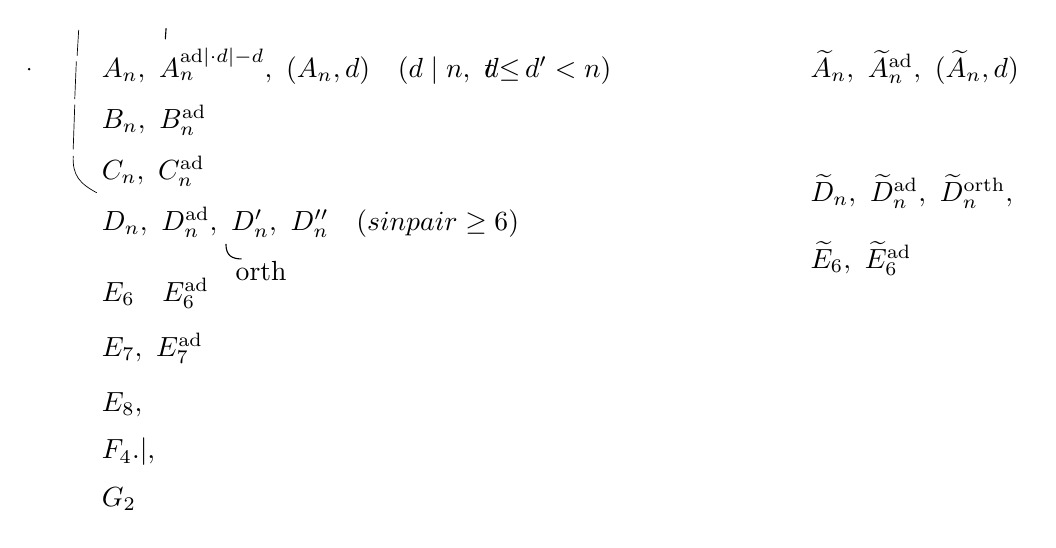
\begin{tikzpicture}[x=1cm,y=1cm]
\draw[line width=.25pt] (-.17,.6)--(-.19,.27);
\draw[line width=.25pt] (-.2,.2)--(-.22,-.28);
\draw[line width=.25pt] (-.22,-.35)--(-.24,-.92);
\draw[line width=.25pt] (-.24,-1) .. controls (-.25,-1.25) and (-.16,-1.35) .. (.06,-1.47);
\fill (-.8,.1) circle (.018cm);
\draw[thin] (.93,.48)--(.94,.62);
\node[anchor=base west] at (0,0) {$A_n,\ A_n^{\unsure{\mathrm{ad}|{\cdot}d|-d}},\ (A_n,d)\quad(d\mid n,\ \unsure{\rlap{$d$}t}\,\unsure{\leq}\,\unsure{d'}<n)$};
\node[anchor=base west] at (0,-.65) {$B_n,\ B_n^{\mathrm{ad}}$};
\node[anchor=base west] at (0,-1.3) {$C_n,\ C_n^{\mathrm{ad}}$};
\node[anchor=base west] at (0,-1.95) {$D_n,\ D_n^{\mathrm{ad}},\ D'_n,\ D''_n\quad(\text{si }n\text{ pair }\geq6)$};
\draw[thin] (1.7,-2.12) .. controls (1.7,-2.27) and (1.78,-2.31) .. (1.9,-2.31);
\node[anchor=base west] at (1.7,-2.58) {orth};
\node[anchor=base west] at (0,-2.85) {$E_6\quad E_6^{\mathrm{ad}}$};
\node[anchor=base west] at (0,-3.55) {$E_7,\ E_7^{\mathrm{ad}}$};
\node[anchor=base west] at (0,-4.25) {$E_8,$};
\node[anchor=base west] at (0,-4.85) {$F_4\unsure{.|,}$};
\node[anchor=base west] at (0,-5.45) {$G_2$};
\node[anchor=base west] at (9,0) {$\widetilde{A}_n,\ \widetilde{A}_n^{\mathrm{ad}},\ (\widetilde{A}_n,d)$};
\node[anchor=base west] at (9,-1.58) {$\widetilde{D}_n,\ \widetilde{D}_n^{\mathrm{ad}},\ \widetilde{D}_n^{\mathrm{orth}},$};
\node[anchor=base west] at (9,-2.43) {$\widetilde{E}_6,\ \widetilde{E}_6^{\mathrm{ad}}$};
\end{tikzpicture}}}

\handwritten{\diagram{\(\begin{array}{lcl}
21\ \text{\uline{cas à examiner}} & \left\{\begin{array}{l}
\text{a) en partant des groupes \unsure{comp. et connexes|compacts connexes|comp. et ce comme} \unsure{gr. p\textsuperscript{r} de réf.|gr. de réf.|gr. de Lie.}}\\[.7em]
\text{b) en partant des Chevalley}
\end{array}\right. &
\end{array}\)}}
\handwritten{\figure{\begin{tikzpicture}
\draw (0,0) -- (2.3,.03) -- (4.2,0) -- (6,.035) -- (8,.01) -- (10,.045) -- (12,.15);
\draw[line width=.3pt] (3.3,.13)--(3.4,.13);
\draw[line width=.3pt] (4.12,.16)--(4.28,.18);
\draw[line width=.3pt] (8.12,-2.4) .. controls (8.2,-2.4) and (8.32,-2.45) .. (8.42,-2.47);
\end{tikzpicture}}}

